\chapter{2 Samuel 23}

\begin{figure}
  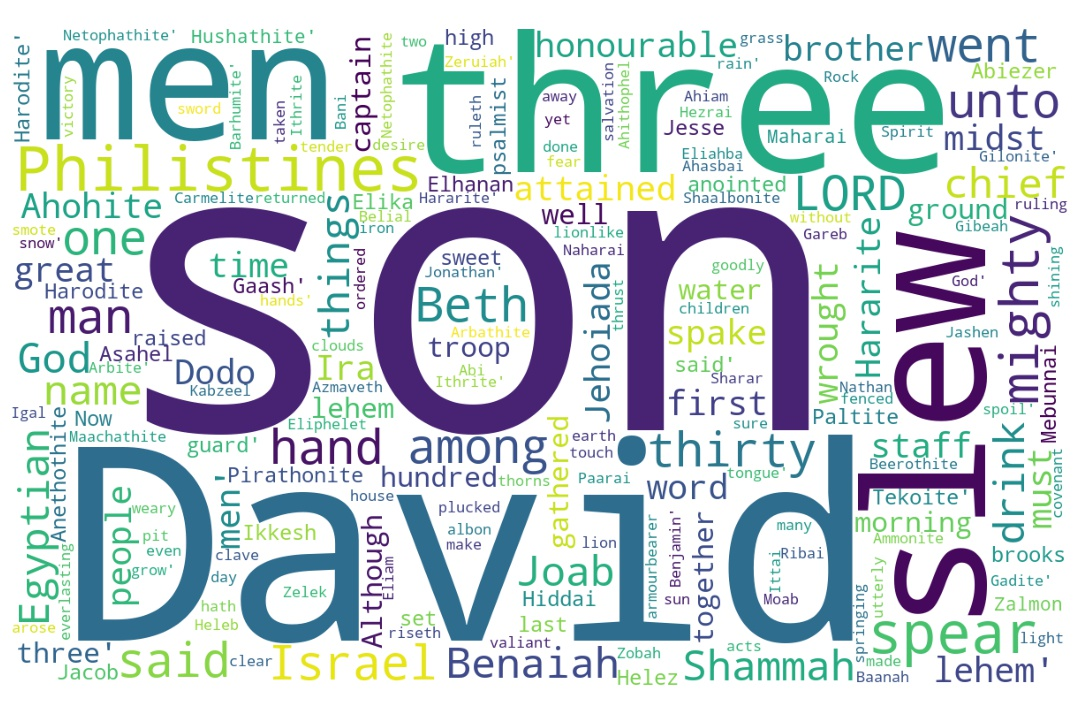
\includegraphics[width=\linewidth]{10OT-2Samuel/2Samuel23-WordCloud.jpg}
  \caption{1 Samuel 23 Word Cloud}
  \label{fig:1 Samuel 23 Word Cloud}
\end{figure}

%%%%%%%%%%%%%%%%%%%%%%%%%%%%%%%%%%%%%%%%%
%%%%%%%%%%%%%%%%%%%%%%%%%%%%%%%%%%%%%%%%%


\marginpar{\scriptsize \centering \fcolorbox{bone}{lime}{\textbf{DAVID"S MIGHTY MEN}}\\ (2 Samuel 23:1--39) 
\begin{compactenum}[I.][8]
    \item A Final  \textbf{Message} \index[scripture]{2Samuel!2Sa 22:01} (2Sa 22:1) 
    \item Things that are  \textbf{Memorable} \index[scripture]{2Samuel!2Sa 22:01} (2Sa 22:1) 
    \item The  \textbf{Mighty} Men \index[scripture]{2Samuel!2Sa 22:01} (2Sa 22:1) 
    \item Those Even  \textbf{More} Special \index[scripture]{2Samuel!2Sa 22:01} (2Sa 22:1) 
    \item A  \textbf{Moment} \index[scripture]{2Samuel!2Sa 23:13--17} (2Sa 23:13--17) 
    \item The  \textbf{Mistake} \index[scripture]{2Samuel!2Sa 23:39} (2Sa 23:39) 
   \item A  \textbf{Message} \index[scripture]{2Samuel!2Sa 23:13--17} (2Sa 23:13--17) 
\end{compactenum} }

\footnote{\textcolor[cmyk]{0.99998,1,0,0}{\hyperlink{TOC}{Return to end of Table of Contents.}}}\footnote{\href{https://audiobible.com/bible/2_samuel_23.html}{\textcolor[cmyk]{0.99998,1,0,0}{2 Samuel 23 Audio}}}\textcolor[cmyk]{0.99998,1,0,0}{Now these \emph{be} the last words of David. David the son of Jesse said, and the man \emph{who} \emph{was} raised up on high, the anointed of the God of Jacob, and the sweet psalmist of Israel, said,}
[2] \textcolor[cmyk]{0.99998,1,0,0}{The Spirit of the LORD spake by me, and his word \emph{was} in my tongue.}
[3] \textcolor[cmyk]{0.99998,1,0,0}{The God of Israel said, the Rock of Israel spake to me, He that ruleth over men \emph{must} \emph{be} just, ruling in the fear of God.}
[4] \textcolor[cmyk]{0.99998,1,0,0}{And \emph{he} \emph{shall} \emph{be} as the light of the morning, \emph{when} the sun riseth, \emph{even} \fcolorbox{bone}{bone}{a}morning without clouds; \emph{as} the tender grass \emph{springing} out of the earth by clear shining after rain.}
[5] \textcolor[cmyk]{0.99998,1,0,0}{Although my house \emph{be} not so with God; yet he hath made with me an everlasting covenant, ordered in all \emph{things}, and sure: for \emph{this} \emph{is} all my salvation, and all \emph{my} desire, although he make \emph{it} not to grow.}\\
\\
\P \textcolor[cmyk]{0.99998,1,0,0}{But \emph{the} \emph{sons} of Belial \emph{shall} \emph{be} all of them as thorns thrust away, because they cannot be taken with hands:}
[7] \textcolor[cmyk]{0.99998,1,0,0}{But the man \emph{that} shall touch them must be fenced with iron and the staff of \fcolorbox{bone}{bone}{a}spear; and they shall be utterly burned with fire in the \emph{same} place.}\\
\\
\P \textcolor[cmyk]{0.99998,1,0,0}{These \emph{be} the names of the mighty men whom David had: The Tachmonite that sat in the seat, chief among the captains; the same \emph{was} Adino the Eznite: \emph{he} \emph{lift} \emph{up} \emph{his} \emph{spear} against eight hundred, whom he slew at one time.}
[9] \textcolor[cmyk]{0.99998,1,0,0}{And after him \emph{was} Eleazar the son of Dodo the Ahohite, \emph{one} of the three mighty men with David, when they defied the Philistines \emph{that} were there gathered together to battle, and the men of Israel were gone away:}
[10] \textcolor[cmyk]{0.99998,1,0,0}{He arose, and smote the Philistines until his hand was weary, and his hand clave unto the sword: and the LORD wrought \fcolorbox{bone}{bone}{a}great victory that day; and the people returned after him only to spoil.}
[11] \textcolor[cmyk]{0.99998,1,0,0}{And after him \emph{was} Shammah the son of Agee the Hararite. And the Philistines were gathered together into \fcolorbox{bone}{bone}{a}troop, where was \fcolorbox{bone}{bone}{a}piece of ground full of lentiles: and the people fled from the Philistines.}
[12] \textcolor[cmyk]{0.99998,1,0,0}{But he stood in the midst of the ground, and defended it, and slew the Philistines: and the LORD wrought \fcolorbox{bone}{bone}{a}great victory.}
[13] \textcolor[cmyk]{0.99998,1,0,0}{And three of the thirty chief went down, and came to David in the harvest time unto the cave of Adullam: and the troop of the Philistines pitched in the valley of Rephaim.}
[14] \textcolor[cmyk]{0.99998,1,0,0}{And David \emph{was} then in an hold, and the garrison of the Philistines \emph{was} then \emph{in} Beth-lehem.}
[15] \textcolor[cmyk]{0.99998,1,0,0}{And David longed, and said, Oh that one would give me drink of the water of the well of Beth-lehem, which \emph{is} by the gate!}
[16] \textcolor[cmyk]{0.99998,1,0,0}{And the three mighty men brake through the host of the Philistines, and drew water out of the well of Beth-lehem, that \emph{was} by the gate, and took \emph{it}, and brought \emph{it} to David: nevertheless he would not drink thereof, but poured it out unto the LORD.}
[17] \textcolor[cmyk]{0.99998,1,0,0}{And he said, Be it far from me, O LORD, that I should do this: \emph{is} \emph{not} \emph{this} the blood of the men that went in jeopardy of their lives? therefore he would not drink it. These things did these three mighty men.}
[18] \textcolor[cmyk]{0.99998,1,0,0}{And Abishai, the brother of Joab, the son of Zeruiah, was chief among three. And he lifted up his spear against three hundred, \emph{and} slew \emph{them}, and had the name among three.}
[19] \textcolor[cmyk]{0.99998,1,0,0}{Was he not most honourable of three? therefore he was their captain: howbeit he attained not unto the \emph{first} three.}
[20] \textcolor[cmyk]{0.99998,1,0,0}{And Benaiah the son of Jehoiada, the son of \fcolorbox{bone}{bone}{a}valiant man, of Kabzeel, who had done many acts, he slew two lionlike men of Moab: he went down also and slew \fcolorbox{bone}{bone}{a}lion in the midst of \fcolorbox{bone}{bone}{a}pit in time of snow:}
[21] \textcolor[cmyk]{0.99998,1,0,0}{And he slew an Egyptian, \fcolorbox{bone}{bone}{a}goodly man: and the Egyptian had \fcolorbox{bone}{bone}{a}spear in his hand; but he went down to him with \fcolorbox{bone}{bone}{a}staff, and plucked the spear out of the Egyptian's hand, and slew him with his own spear.}
[22] \textcolor[cmyk]{0.99998,1,0,0}{These \emph{things} did Benaiah the son of Jehoiada, and had the name among three mighty men.}
[23] \textcolor[cmyk]{0.99998,1,0,0}{He was more honourable than the thirty, but he attained not to the \emph{first} three. And David set him over his guard.}
[24] \textcolor[cmyk]{0.99998,1,0,0}{Asahel the brother of Joab \emph{was} one of the thirty; Elhanan the son of Dodo of Beth-lehem,}
[25] \textcolor[cmyk]{0.99998,1,0,0}{Shammah the Harodite, Elika the Harodite,}
[26] \textcolor[cmyk]{0.99998,1,0,0}{Helez the Paltite, Ira the son of Ikkesh the Tekoite,}
[27] \textcolor[cmyk]{0.99998,1,0,0}{Abiezer the Anethothite, Mebunnai the Hushathite,}
[28] \textcolor[cmyk]{0.99998,1,0,0}{Zalmon the Ahohite, Maharai the Netophathite,}
[29] \textcolor[cmyk]{0.99998,1,0,0}{Heleb the son of Baanah, \fcolorbox{bone}{bone}{a}Netophathite, Ittai the son of Ribai out of Gibeah of the children of Benjamin,}
[30] \textcolor[cmyk]{0.99998,1,0,0}{Benaiah the Pirathonite, Hiddai of the brooks of Gaash,}
[31] \textcolor[cmyk]{0.99998,1,0,0}{Abi-albon the Arbathite, Azmaveth the Barhumite,}
[32] \textcolor[cmyk]{0.99998,1,0,0}{Eliahba the Shaalbonite, of the sons of Jashen, Jonathan,}
[33] \textcolor[cmyk]{0.99998,1,0,0}{Shammah the Hararite, Ahiam the son of Sharar the Hararite,}
[34] \textcolor[cmyk]{0.99998,1,0,0}{Eliphelet the son of Ahasbai, the son of the Maachathite, Eliam the son of Ahithophel the Gilonite,}
[35] \textcolor[cmyk]{0.99998,1,0,0}{Hezrai the Carmelite, Paarai the Arbite,}
[36] \textcolor[cmyk]{0.99998,1,0,0}{Igal the son of Nathan of Zobah, Bani the Gadite,}
[37] \textcolor[cmyk]{0.99998,1,0,0}{Zelek the Ammonite, Naharai the Beerothite, armourbearer to Joab the son of Zeruiah,}
[38] \textcolor[cmyk]{0.99998,1,0,0}{Ira an Ithrite, Gareb an Ithrite,}
[39] \textcolor[cmyk]{0.99998,1,0,0}{Uriah the Hittite: thirty and seven in all.}